\section{Evaluation}

The evaluation of our work is executed on a discrete-event simulator written in Python. This simulator is similar to existing discrete-event simulators such as ns3. Events are put onto a priority queue ordered by time, and executed in a single loop.

This simulator takes in as input different network structures with a list of nodes, links, and node types. 
Nodes can be either honest or malicious. As mentioned before, we simulate passive adversaries: malicious nodes are honest-but-curious. Whenever a malicious node receives a message, it adds the message, along with the time at which the message is received, to a list of intercepted messages. The timestamp used is the global simulator time, thus we assume that the spies' clocks are roughly synchronized (or that the synchronization time is much smaller than). 

At the start of a simulation run, a certain percentage of the nodes are compromised. The percentage number can be tweaked to adjust the number of malicious nodes in the network. The simulator then runs for some number of time steps and produces a list of messages intercepted from malicious nodes. After the simulation, the estimators take in the list of timestamped messages and produce guesses for the true source of the message.

\subsection{Estimator validation}
We started by attempting to replicate the estimator results in \cite{pinto}. 
In this replication process, we ran into a number of challenges. We encountered four primary mistakes or omissions in \cite{pinto} that affected our estimation accuracy; some of these were easy to correct once we identified them, others were not:
\begin{itemize}
\item There is a typo in equation (2), which describes how to compute the observed delay vector. It should say $[\boldsymbol d]_k=t_{k+1}-t_1$ instead of $[\boldsymbol d]_k=t_{k+1}-t_k$. This is a critical mistake in the description of the estimator that leads to incorrect likelihoods. 
\item Algorithm 2 of the supplemental materials describes how to compute likelihoods for general graphs. In step 6, it should say ``compute the source likelihood using equation (4) for node $s$.", rather than ``using equation (7)." This is because over general graphs, the covariance matrix $\Lambda_s$ is not identical for all nodes, which causes the simplifications in equation (7) to be invalid. As such, the likelihoods should be computed using the more general equation (4). This error initially led to incorrect likelihood computations in our code.
\item Algorithm 2 of the supplemental materials does not explain how to prune graphs that are not tree-structured. Additionally, it does not describe how to incorporate the direction of infection into estimation. These omissions collectively have a significant impact the likelihoods obtained by the algorithm, and we suspect this is partially responsible for our inability to exactly reproduce their results.
\item The parameter specifications of the random graphs in Table 1 are not given. Specifically, the Barabasi-Albert parameter is not given. We therefore tried a range of different parameters.
\end{itemize}

\subsubsection{Trees}
We first tested the estimator on trees. As assumed in \cite{pinto}, each node transmits the message to its neighbors with an iid delay that is distributed according to $\mathcal N(2,0.5)$.
\begin{figure}
\centering
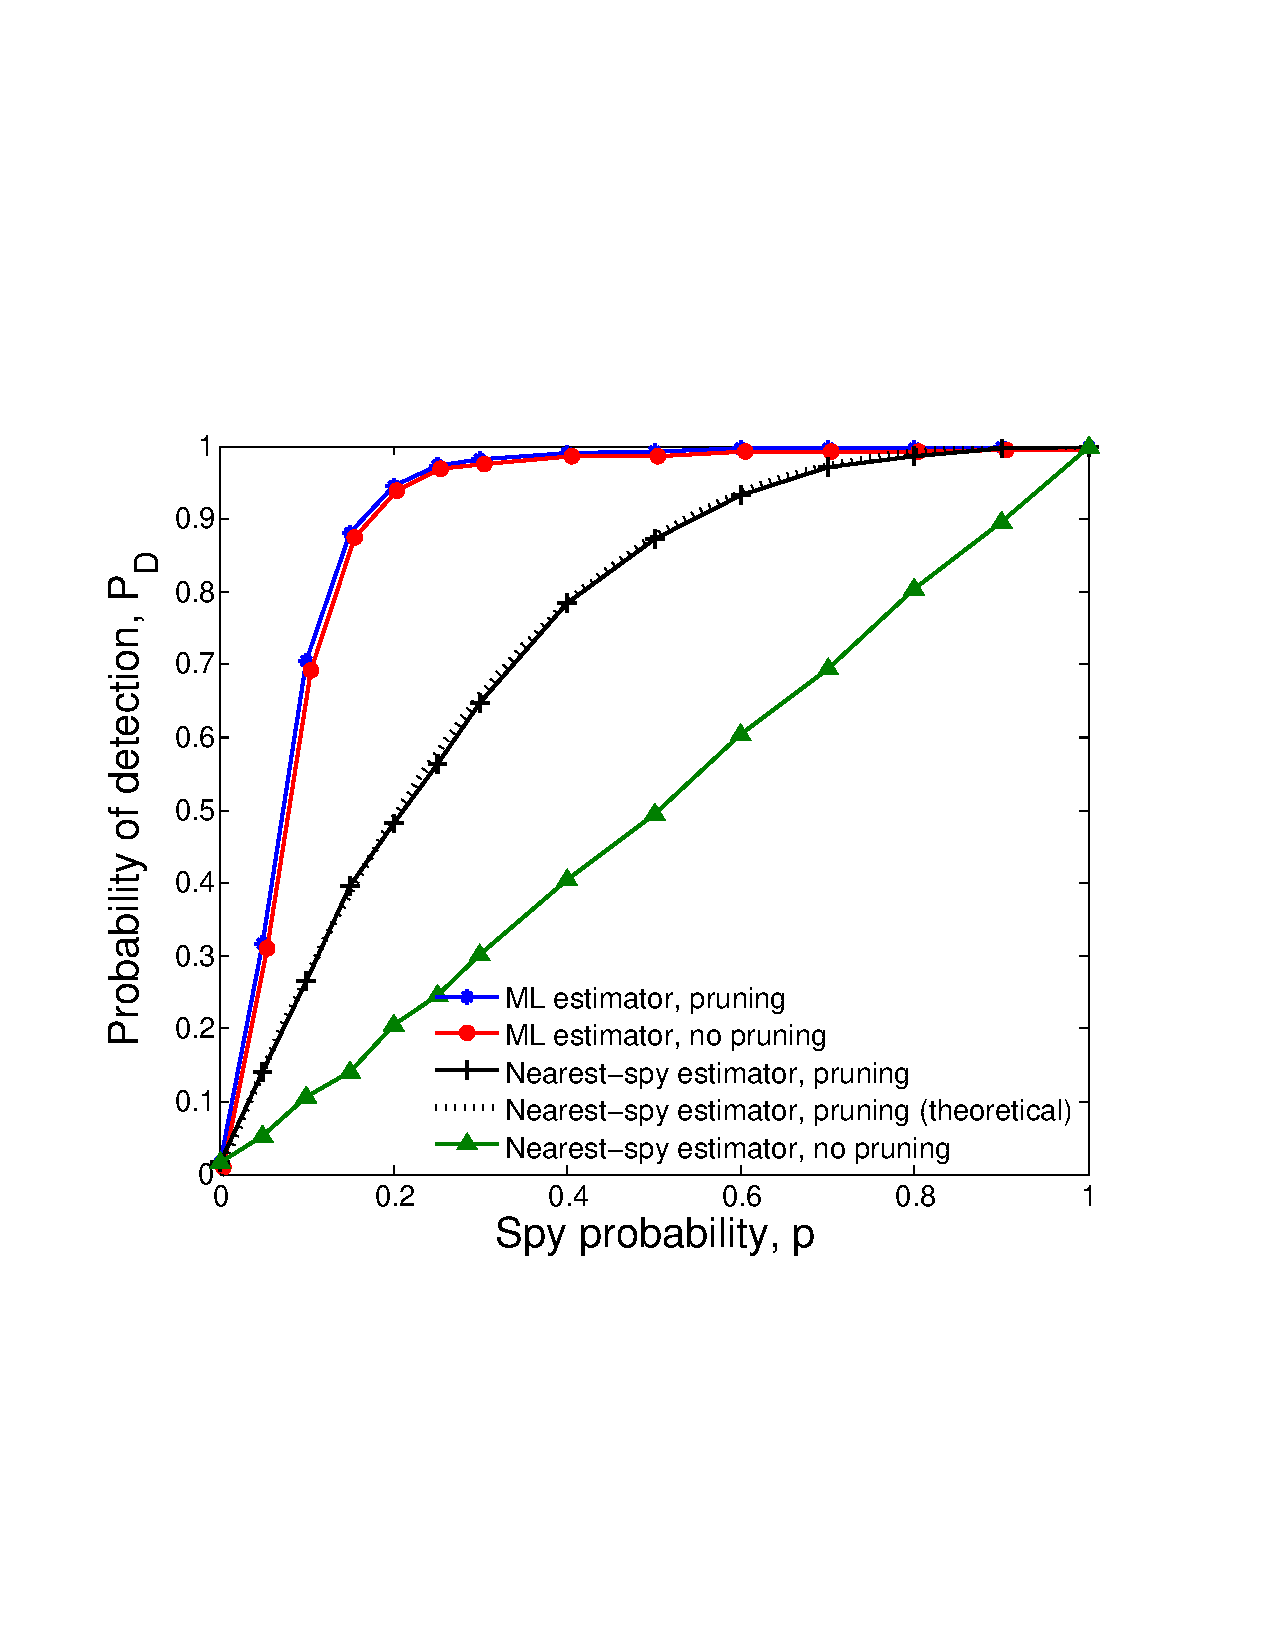
\includegraphics[height = 2.4in]{figures/pd_vs_spies}
\caption{Probability of detection, i.e. $P(\hat v = v^*)$, as a function of the spy probability $p$. This plot was generated over 3-regular trees. Delays $\theta_{ij}$ are modeled as Gaussians $\mathcal N(2,0.5)$, and spreading was run for 8 time units.}
\label{fig:pd_vs_spies}
%\vspace*{-0.4in}
\end{figure}

\begin{figure}
\centering
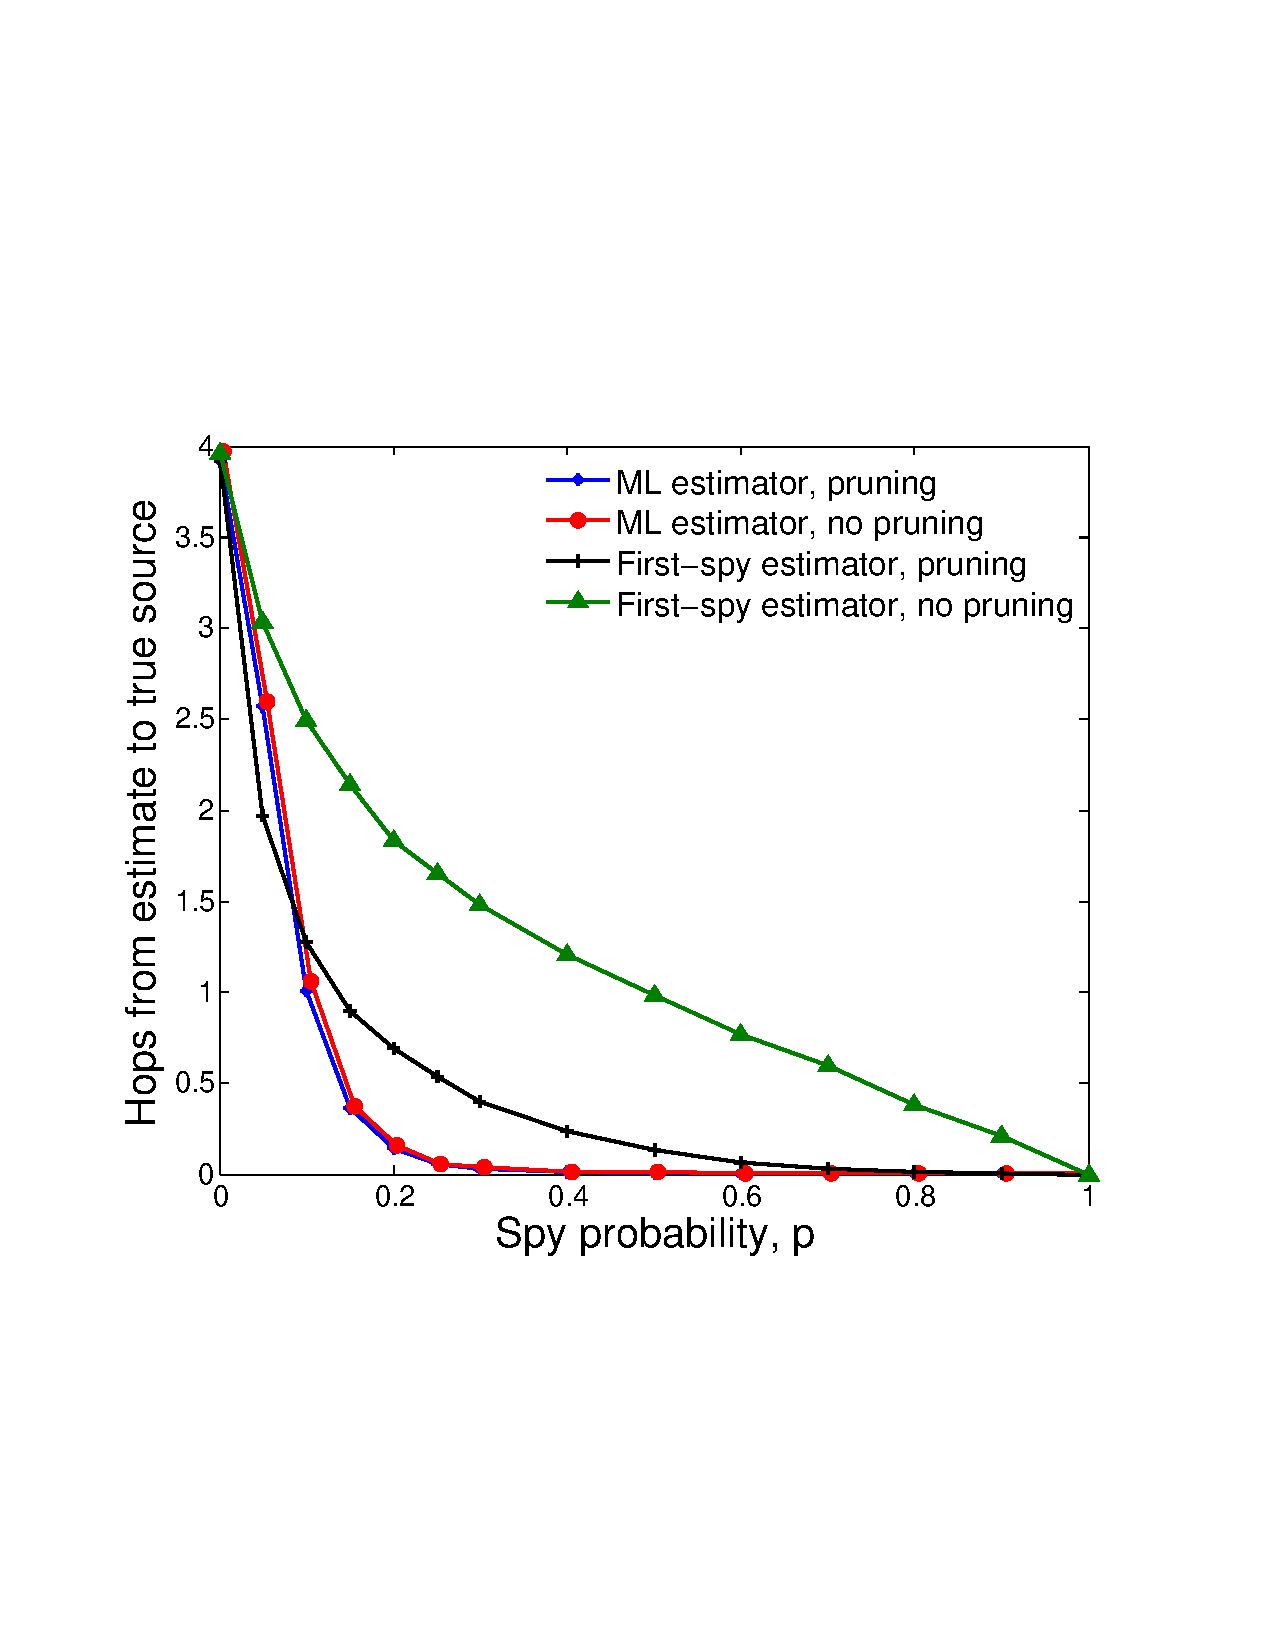
\includegraphics[height = 2.4in]{figures/hops_vs_spies}
\caption{Hop distance of the estimate $\hat v$ from the true source $v^*$ as a function of the spy probability $p$. This plot was generated over 3-regular trees. Delays $\theta_{ij}$ are modeled as Gaussians $\mathcal N(2,0.5)$, and spreading was run for 8 time units.}
\label{fig:pd_vs_spies}
%\vspace*{-0.4in}
\end{figure}

\subsection{Facebook dataset}

Randomized graphs provide decent estimates for the estimators' effectivness, but they are still different from real datasets. In order to test our estimators on realistic data, we use a Facebook dataset~\cite{viswanath-2009-activity} from New Orleans. The dataset contains all of the user-to-user connections on Facebook in New Orleans. Since the number of users is large, we use \emph{ego sampling} on the dataset. Ego sampling takes a random node from the graph and samples all nodes within $n$ hops from the initial node. For our experiments, we use $n = 2$.
